\chapter{Lampiran B. Tabel dan Tangkapan Layar Hasil Pengujian Kinerja}
\label{lampiran_b}

% Please add the following required packages to your document preamble:
% \usepackage[table,xcdraw]{xcolor}
% If you use beamer only pass "xcolor=table" option, i.e. \documentclass[xcolor=table]{beamer}
\begin{table}[!htb]
	\caption{Tabel hasil pengujian kinerja}
	\centering
	\begin{tabular}{|l|c|c|}
		\hline
		\rowcolor[HTML]{6434FC} 
		{\color[HTML]{FFFFFF} ID} &
		\multicolumn{1}{l|}{\cellcolor[HTML]{6434FC}{\color[HTML]{FFFFFF} CPU (vCPU)}} &
		\multicolumn{1}{l|}{\cellcolor[HTML]{6434FC}{\color[HTML]{FFFFFF} Memory (MiB)}} \\ \hline
		\textbf{SI1}     & 0,042 & 137,82  \\ \hline
		\textbf{SI2}     & 0,043 & 128,71  \\ \hline
		\textbf{SI3}     & 0,04  & 131,55  \\ \hline
		\textbf{SI4}     & 0,045 & 146,6   \\ \hline
		\textbf{SI5}     & 0,046 & 153,61  \\ \hline
		\textbf{SI6}     & 0,047 & 152,71  \\ \hline
		\textbf{SI7}     & 0,048 & 152,71  \\ \hline
		\textbf{SE1}     & 0,049 & 168,8   \\ \hline
		\textbf{SE2}     & 0,05  & 183,68  \\ \hline
		\textbf{SE3}     & 0,051 & 176,59  \\ \hline
		\textbf{SE4}     & 0,052 & 165,75  \\ \hline
		\textbf{Average} & 0,046 & 154,411 \\ \hline
		\textbf{STD}     & 0,038 & 17,916  \\ \hline
	\end{tabular}
\end{table}

\begin{figure}[!htb]
	\centering
	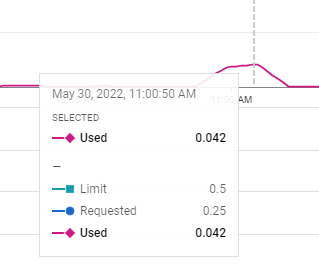
\includegraphics[width=0.5\textwidth]{resources/ch4/resource/1-cpu.png}
	\caption{Penggunaan CPU pada kasus \textbf{SI1}}
	\label{result_cpu_1}
\end{figure}

\begin{figure}[!htb]
	\centering
	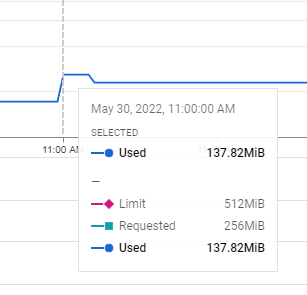
\includegraphics[width=0.5\textwidth]{resources/ch4/resource/1-mem.png}
	\caption{Penggunaan Memory pada kasus \textbf{SI1}}
	\label{result_mem_1}
\end{figure}

\begin{figure}[!htb]
	\centering
	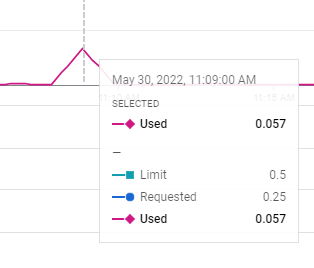
\includegraphics[width=0.5\textwidth]{resources/ch4/resource/2-cpu.png}
	\caption{Penggunaan CPU pada kasus \textbf{SI2}}
	\label{result_cpu_2}
\end{figure}

\begin{figure}[!htb]
	\centering
	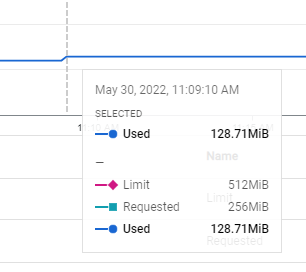
\includegraphics[width=0.5\textwidth]{resources/ch4/resource/2-mem.png}
	\caption{Penggunaan Memory pada kasus \textbf{SI2}}
	\label{result_mem_2}
\end{figure}

\begin{figure}[!htb]
	\centering
	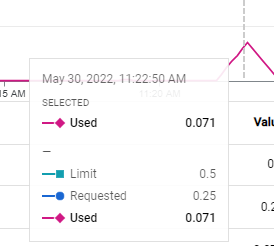
\includegraphics[width=0.5\textwidth]{resources/ch4/resource/3-cpu.png}
	\caption{Penggunaan CPU pada kasus \textbf{SI3}}
	\label{result_cpu_3}
\end{figure}

\begin{figure}[!htb]
	\centering
	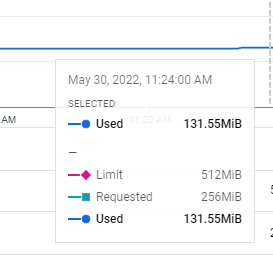
\includegraphics[width=0.5\textwidth]{resources/ch4/resource/3-mem.png}
	\caption{Penggunaan Memory pada kasus \textbf{SI3}}
	\label{result_mem_3}
\end{figure}

\begin{figure}[!htb]
	\centering
	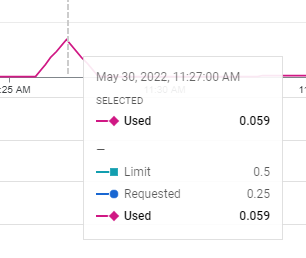
\includegraphics[width=0.5\textwidth]{resources/ch4/resource/4-cpu.png}
	\caption{Penggunaan CPU pada kasus \textbf{SI4}}
	\label{result_cpu_4}
\end{figure}

\begin{figure}[!htb]
	\centering
	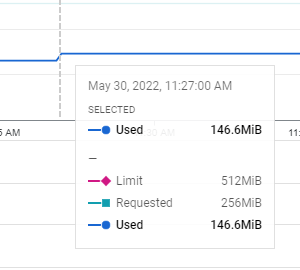
\includegraphics[width=0.5\textwidth]{resources/ch4/resource/4-mem.png}
	\caption{Penggunaan Memory pada kasus \textbf{SI4}}
	\label{result_mem_4}
\end{figure}

\begin{figure}[!htb]
	\centering
	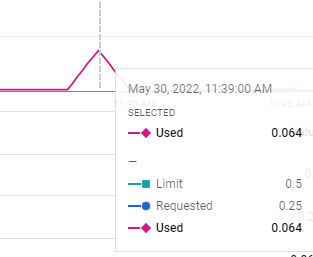
\includegraphics[width=0.5\textwidth]{resources/ch4/resource/5-cpu.png}
	\caption{Penggunaan CPU pada kasus \textbf{SI5}}
	\label{result_cpu_5}
\end{figure}

\begin{figure}[!htb]
	\centering
	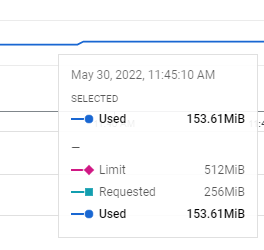
\includegraphics[width=0.5\textwidth]{resources/ch4/resource/5-mem.png}
	\caption{Penggunaan Memory pada kasus \textbf{SI5}}
	\label{result_mem_5}
\end{figure}

\begin{figure}[!htb]
	\centering
	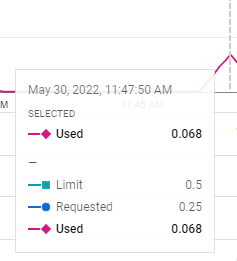
\includegraphics[width=0.5\textwidth]{resources/ch4/resource/6-cpu.png}
	\caption{Penggunaan CPU pada kasus \textbf{SI6}}
	\label{result_cpu_6}
\end{figure}

\begin{figure}[!htb]
	\centering
	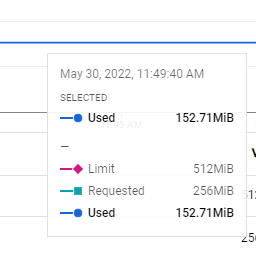
\includegraphics[width=0.5\textwidth]{resources/ch4/resource/6-mem.png}
	\caption{Penggunaan Memory pada kasus \textbf{SI6}}
	\label{result_mem_6}
\end{figure}

\begin{figure}[!htb]
	\centering
	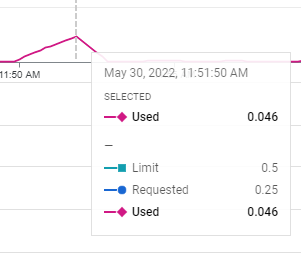
\includegraphics[width=0.5\textwidth]{resources/ch4/resource/7-cpu.png}
	\caption{Penggunaan CPU pada kasus \textbf{SI7}}
	\label{result_cpu_7}
\end{figure}

\begin{figure}[!htb]
	\centering
	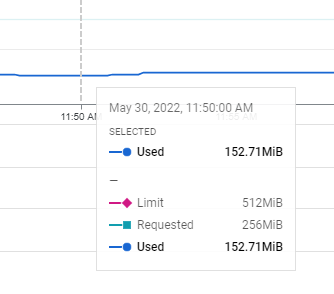
\includegraphics[width=0.5\textwidth]{resources/ch4/resource/7-mem.png}
	\caption{Penggunaan Memory pada kasus \textbf{SI7}}
	\label{result_mem_7}
\end{figure}

\begin{figure}[!htb]
	\centering
	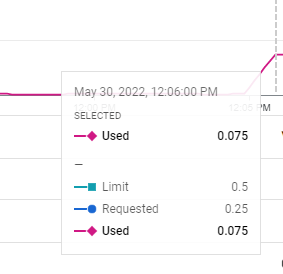
\includegraphics[width=0.5\textwidth]{resources/ch4/resource/8-cpu.png}
	\caption{Penggunaan CPU pada kasus \textbf{SE1}}
	\label{result_cpu_8}
\end{figure}

\begin{figure}[!htb]
	\centering
	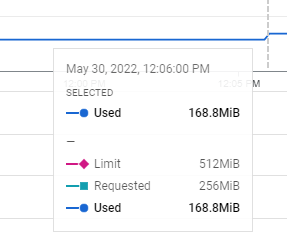
\includegraphics[width=0.5\textwidth]{resources/ch4/resource/8-mem.png}
	\caption{Penggunaan Memory pada kasus \textbf{SE1}}
	\label{result_mem_8}
\end{figure}

\begin{figure}[!htb]
	\centering
	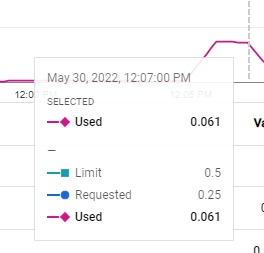
\includegraphics[width=0.5\textwidth]{resources/ch4/resource/9-cpu.png}
	\caption{Penggunaan CPU pada kasus \textbf{SE2}}
	\label{result_cpu_9}
\end{figure}

\begin{figure}[!htb]
	\centering
	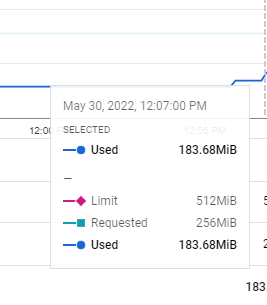
\includegraphics[width=0.5\textwidth]{resources/ch4/resource/9-mem.png}
	\caption{Penggunaan Memory pada kasus \textbf{SE2}}
	\label{result_mem_9}
\end{figure}

\begin{figure}[!htb]
	\centering
	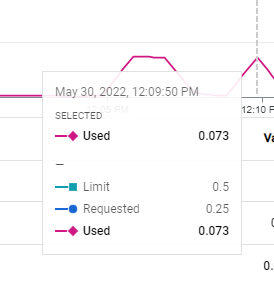
\includegraphics[width=0.5\textwidth]{resources/ch4/resource/10-cpu.png}
	\caption{Penggunaan CPU pada kasus \textbf{SE3}}
	\label{result_cpu_10}
\end{figure}

\begin{figure}[!htb]
	\centering
	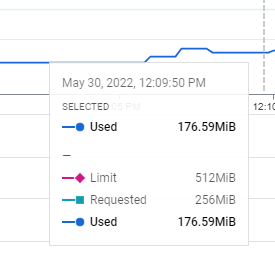
\includegraphics[width=0.5\textwidth]{resources/ch4/resource/10-mem.png}
	\caption{Penggunaan Memory pada kasus \textbf{SE3}}
	\label{result_mem_10}
\end{figure}

\begin{figure}[!htb]
	\centering
	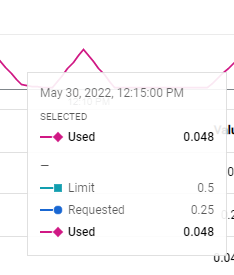
\includegraphics[width=0.5\textwidth]{resources/ch4/resource/11-cpu.png}
	\caption{Penggunaan CPU pada kasus \textbf{SE4}}
	\label{result_cpu_11}
\end{figure}

\begin{figure}[!htb]
	\centering
	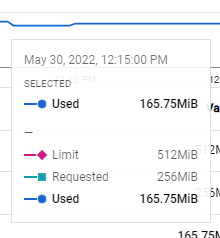
\includegraphics[width=0.5\textwidth]{resources/ch4/resource/11-mem.png}
	\caption{Penggunaan Memory pada kasus \textbf{SE4}}
	\label{result_mem_11}
\end{figure}